\documentclass[tikz,border=3mm,multi=tikzpicture]{standalone}
\usepackage{tikz}
\usetikzlibrary{arrows.meta,positioning}
\begin{document}

% TikZ 1
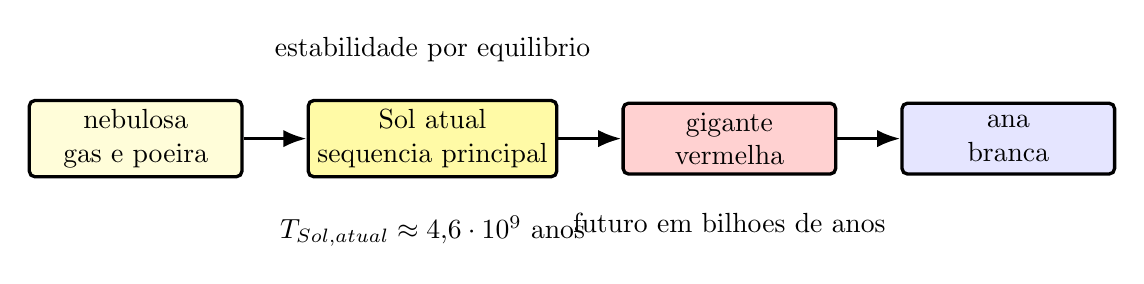
\begin{tikzpicture}[>=Latex,node distance=0.7cm]
  \tikzstyle{fase}=[draw,rounded corners=2pt,minimum width=2.7cm,minimum height=0.9cm,align=center,very thick]
  \node[fase,fill=yellow!15] (nuvem) {nebulosa\\gas e poeira};
  \node[fase,fill=yellow!35,right=0.8cm of nuvem] (seq) {Sol atual\\sequencia principal};
  \node[fase,fill=red!18,right=0.8cm of seq] (gig) {gigante\\vermelha};
  \node[fase,fill=blue!10,right=0.8cm of gig] (ana) {ana\\branca};
  \draw[very thick,->] (nuvem) -- (seq);
  \draw[very thick,->] (seq) -- (gig);
  \draw[very thick,->] (gig) -- (ana);
  \node[below=0.35cm of seq,align=center] {$T_{Sol,atual}\approx4{,}6\cdot10^9\ \mathrm{anos}$};
  \node[above=0.35cm of seq,align=center] {estabilidade por equilibrio};
  \node[below=0.35cm of gig,align=center] {futuro em bilhoes de anos};
\end{tikzpicture}

% TikZ 2
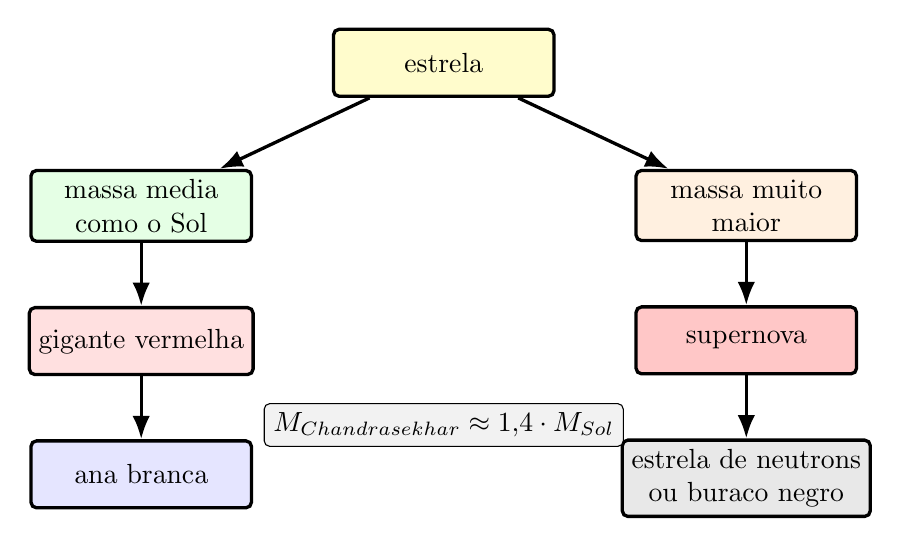
\begin{tikzpicture}[>=Latex,node distance=0.75cm]
  \tikzstyle{box}=[draw,rounded corners=2pt,minimum width=2.8cm,minimum height=0.85cm,align=center,very thick]
  \node[box,fill=yellow!20] (estrela) {estrela};
  \node[box,fill=green!10,below left=0.9cm and 1cm of estrela] (media) {massa media\\como o Sol};
  \node[box,fill=orange!12,below right=0.9cm and 1cm of estrela] (massiva) {massa muito\\maior};
  \node[box,fill=red!12,below=0.8cm of media] (gv) {gigante vermelha};
  \node[box,fill=blue!10,below=0.8cm of gv] (ab) {ana branca};
  \node[box,fill=red!22,below=0.8cm of massiva] (sn) {supernova};
  \node[box,fill=gray!18,below=0.8cm of sn] (final) {estrela de neutrons\\ou buraco negro};
  \draw[very thick,->] (estrela) -- (media);
  \draw[very thick,->] (estrela) -- (massiva);
  \draw[very thick,->] (media) -- (gv);
  \draw[very thick,->] (gv) -- (ab);
  \draw[very thick,->] (massiva) -- (sn);
  \draw[very thick,->] (sn) -- (final);
  \node[draw,rounded corners=2pt,fill=gray!10,align=center] at (0,-4.6)
    {$M_{Chandrasekhar}\approx1{,}4\cdot M_{Sol}$};
\end{tikzpicture}

\end{document}
